\section{Results}
\label{sec:results}

\begin{figure}[t]
\centering
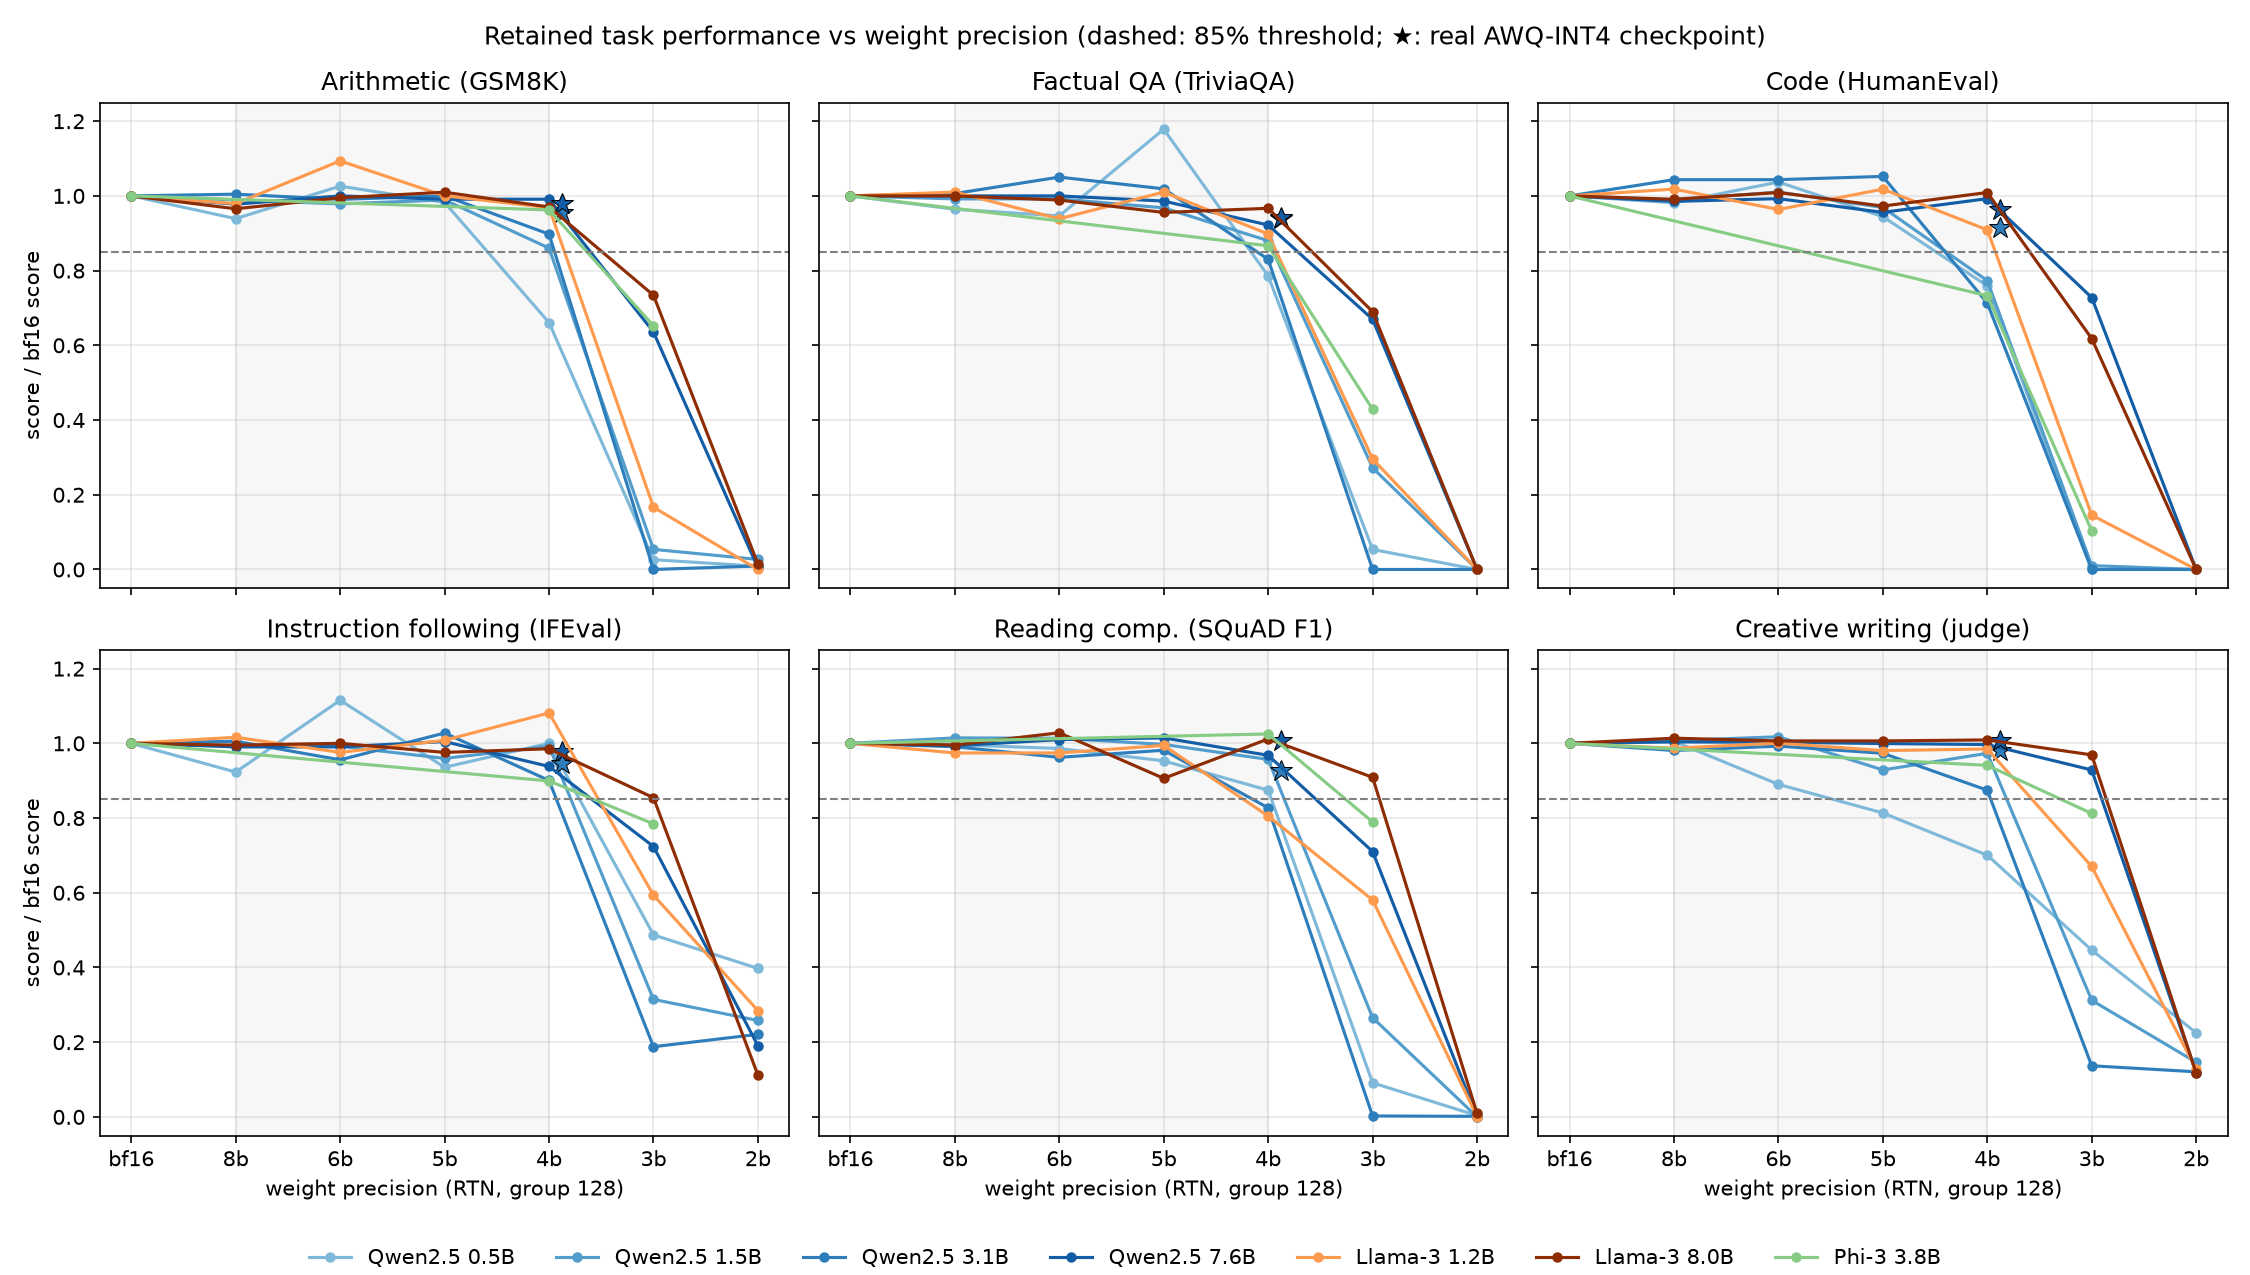
\includegraphics[width=0.95\linewidth]{figures/fig1_retained_vs_bits.png}
\caption{Retained score (quantized / bf16) as weight precision drops, for each task type. Lines show \rtn group-128 per model, and stars mark official \awq INT4 checkpoints. The dashed line marks 0.85 retained, and the grey band spans INT8$\to$INT4. All curves are flat from 8 to 5 bits. Most curves drop sharply between 4 and 3 bits, and the 7--8B models (dark lines) drop mainly between 3 and 2 bits. \awq stars sit close to 1.0 at 4 bits even when \rtn INT4 does not.}
\label{fig:retained}
\end{figure}

We organize the results around the four hypotheses. \Secref{sec:cliff} locates the cliff and ranks tasks (H1, H2), \secref{sec:errors} examines what quantization errors look like, \secref{sec:size} tests the effect of model size (H3), \secref{sec:kl} tests KL as an early warning (H4), and \secref{sec:granularity} ablates quantization granularity. \Tabref{tab:bf16} in the appendix lists the bf16 reference scores with confidence intervals.

\subsection{Where is the cliff? (H1, H2)}
\label{sec:cliff}

\begin{table}[t]
\centering
\caption{Mean retained fraction across models (\rtn, group 128), with the number of models showing a significant drop vs.\ bf16 (paired test, BH-corrected $q<0.05$) in small type. Six models are tested at 8/6/5/2 bits and seven at 4/3 bits. The most robust task at each of 4, 3 and 2 bits is in \textbf{bold}, and the most fragile is \underline{underlined}. $^\dagger$\ifeval has a non-zero floor, because degenerate output trivially satisfies some constraints.}
\label{tab:retained}
\resizebox{\textwidth}{!}{%
\begin{tabular}{@{}lcccccc@{}}
\toprule
\textbf{Task} & \textbf{8 bits} & \textbf{6 bits} & \textbf{5 bits} & \textbf{4 bits} & \textbf{3 bits} & \textbf{2 bits} \\
\midrule
Arithmetic (\gsm) & 0.98 {\scriptsize 0/6} & 1.01 {\scriptsize 0/6} & 1.00 {\scriptsize 0/6} & 0.90 {\scriptsize 3/7} & 0.32 {\scriptsize 7/7} & 0.01 {\scriptsize 6/6} \\
Factual QA (\trivia) & 1.00 {\scriptsize 0/6} & 0.99 {\scriptsize 0/6} & 1.02 {\scriptsize 1/6} & 0.88 {\scriptsize 3/7} & 0.34 {\scriptsize 7/7} & \underline{0.00} {\scriptsize 6/6} \\
Code (\humaneval) & 1.00 {\scriptsize 0/6} & 1.01 {\scriptsize 0/6} & 0.99 {\scriptsize 0/6} & \underline{0.84} {\scriptsize 3/7} & \underline{0.23} {\scriptsize 7/7} & \underline{0.00} {\scriptsize 6/6} \\
Instruction following (\ifeval) & 0.99 {\scriptsize 0/6} & 1.00 {\scriptsize 0/6} & 0.99 {\scriptsize 0/6} & \textbf{0.97} {\scriptsize 0/7} & 0.56 {\scriptsize 7/7} & \textbf{0.24}$^\dagger$ {\scriptsize 6/6} \\
Reading comp. (\squad F1) & 0.99 {\scriptsize 1/6} & 1.00 {\scriptsize 1/6} & 0.97 {\scriptsize 1/6} & 0.92 {\scriptsize 5/7} & 0.48 {\scriptsize 7/7} & \underline{0.00} {\scriptsize 6/6} \\
Creative writing (judge) & 1.00 {\scriptsize 0/6} & 0.99 {\scriptsize 1/6} & 0.95 {\scriptsize 2/6} & 0.93 {\scriptsize 3/7} & \textbf{0.61} {\scriptsize 7/7} & 0.14 {\scriptsize 6/6} \\
\bottomrule
\end{tabular}}
\end{table}

\para{8 to 5 bits are essentially lossless.} \Tabref{tab:retained} shows that mean retained scores stay between 0.95 and 1.02 from 8 to 5 bits for every task. At 8 and 6 bits only 3 of 72 paired model--task tests show a significant drop (one small \squad dip at 8 bits; one \squad and one creative-writing drop at 6 bits). At 5 bits, 4 of 36 tests are significant. INT8 is statistically indistinguishable from bf16 on every task except one small \squad dip.

\para{The steepest drop is at 4$\to$3 bits, not INT8$\to$INT4.} For models up to 3.8B, the largest single-step drop occurs at 4$\to$3 bits in 28 of 30 model--task cells; the exceptions are \llama-1B on reading and creative writing. For the 7--8B models it occurs at 3$\to$2 bits in all 12 cells. The pre-registered INT8$\to$INT4 cliff ($>$0.15 retained drop, among the 6 models with both levels) is rare: it appears for 1 of 6 models on arithmetic (\qwen-0.5B), 2 of 6 on factual QA, 3 of 6 on code, 2 of 6 on reading, 1 of 6 on creative writing and 0 of 6 on instruction following. \textbf{H1 is not supported as stated.}

\para{Code, not arithmetic, is most sensitive at INT4.} Arithmetic and factual QA are among the more sensitive tasks at 4 bits (mean retained 0.90 and 0.88, with significant drops in 3 of 7 models each). Code generation, however, is the most sensitive: mean retained is 0.84, and four models (\qwen-0.5B/1.5B/3B and \phithree) keep only 0.71--0.77 of their bf16 pass@1. The INT4 task ranking is not statistically significant (Friedman $p=0.11$). At 3 bits the ranking is clear (Friedman $p=10^{-4}$): code collapses hardest (0.23), followed by arithmetic (0.32), factual QA (0.34) and reading (0.48), while instruction following (0.56) and creative writing (0.61) degrade least.

\para{Reading and creative writing are robust at INT4, except for the smallest model.} Reading comprehension keeps $\ge$0.85 of its bf16 F1 at INT4 for 5 of 7 models, with \llama-1B (0.81) and \qwen-3B (0.83) just below. The \squad drops are small but consistent, so they reach significance more often than for any other task (5 of 7 models). Creative writing is robust at INT4 for all models from 1.2B up (0.87--1.01 retained). \qwen-0.5B, however, degrades gradually from 6 bits (0.89, 0.81, 0.70 at 6, 5, 4 bits). This is the only configuration that falls below 0.85 at a precision above 4 bits. \textbf{H2 is partially supported.}

\para{A better quantizer recovers most of the INT4 loss.} The official \awq INT4 checkpoints retain 0.91--0.98 on every task for \qwen-3B and 0.94--1.01 for \qwen-7B (\tabref{tab:pertask} in the appendix). For \qwen-3B, \awq raises code from 0.71 to 0.91, arithmetic from 0.90 to 0.95, and factual QA from 0.83 to 0.94. With a production quantizer, INT4 is close to lossless for models of 3B and larger.

\subsection{What do quantization errors look like?}
\label{sec:errors}

\begin{table}[t]
\centering
\caption{Answer flips relative to bf16, pooled over models. \emph{Lost} counts items correct in bf16 but wrong after quantization, and \emph{gained} counts the reverse. \emph{Fluent} is the share of lost items whose output terminated normally, \ie without a repetition loop or hitting the token limit. Rows pool different model subsets per level (\phithree only at 4/3 bits). Below 4 bits, losses far exceed gains, and the errors change from fluent to degenerate.}
\label{tab:flips}
\resizebox{\textwidth}{!}{%
\begin{tabular}{@{}lcccccccccccc@{}}
\toprule
& \multicolumn{3}{c}{\textbf{8 bits}} & \multicolumn{3}{c}{\textbf{5 bits}} & \multicolumn{3}{c}{\textbf{4 bits}} & \multicolumn{3}{c}{\textbf{3 bits}} \\
\cmidrule(lr){2-4} \cmidrule(lr){5-7} \cmidrule(lr){8-10} \cmidrule(lr){11-13}
\textbf{Task} & Lost & Gained & Fluent & Lost & Gained & Fluent & Lost & Gained & Fluent & Lost & Gained & Fluent \\
\midrule
Arithmetic & 63 (6\%) & 41 & 0.86 & 112 (11\%) & 108 & 0.93 & 211 (17\%) & 105 & 0.90 & 827 (66\%) & 34 & 0.30 \\
Factual QA & 17 (2\%) & 16 & 1.00 & 80 (9\%) & 75 & 1.00 & 214 (19\%) & 95 & 1.00 & 698 (61\%) & 46 & 0.68 \\
Code & 16 (3\%) & 17 & 1.00 & 58 (10\%) & 50 & 0.95 & 162 (24\%) & 58 & 0.93 & 506 (74\%) & 11 & 0.42 \\
Instruction following & 76 (8\%) & 69 & 0.87 & 139 (15\%) & 131 & 0.82 & 204 (19\%) & 165 & 0.73 & 557 (53\%) & 117 & 0.38 \\
Reading comp. & 29 (1\%) & 17 & 0.90 & 131 (7\%) & 88 & 0.93 & 309 (14\%) & 141 & 0.92 & 1274 (57\%) & 68 & 0.49 \\
\bottomrule
\end{tabular}}
\end{table}

\para{Accuracy hides churn.} \Tabref{tab:flips} shows that at 5 bits, where net accuracy is flat, 7--15\% of the items solved in bf16 are answered wrongly, and a similar number of new items become correct. The quantized model has about the same average accuracy as the original, but it gives different answers to many individual items. Even at 8 bits, 6\% of correct arithmetic answers and 8\% of satisfied \ifeval prompts flip.

\para{INT4 errors are silent; INT3 errors are loud.} At 4 bits, 90--100\% of lost arithmetic, factual QA, code and reading items are fluent, confident wrong answers. Typical factual QA examples are: the founder of the World Cup, \emph{Jules Rimet} $\to$ \emph{Jules Renard}; the top album of 1985 alongside \emph{Like A Virgin}, \emph{Madonna} $\to$ \emph{Michael Jackson}; the run of Star Trek: The Original Series, 3 $\to$ 4 years. Errors like these are hard to catch without labels. At 3 bits most failures are degenerate instead (only 30--68\% fluent): repetition loops that hit the token limit, or truncated rambling. Such failures are easy to detect automatically.

\subsection{Does size protect? (H3)}
\label{sec:size}

\begin{table}[t]
\centering
\caption{Critical precision $\bcrit$: the highest tested bit width at which the model keeps less than 85\% of its bf16 score; lower is more robust. Models are sorted by size. Cells at 4 bits or above are in \textbf{bold}. \phithree was tested only at bf16/4/3 bits.}
\label{tab:critical}
\begin{tabular}{@{}lrccccccc@{}}
\toprule
\textbf{Model} & \textbf{Params} & \textbf{Arith.} & \textbf{Fact.\ QA} & \textbf{Code} & \textbf{Instr.} & \textbf{Reading} & \textbf{Creative} & \textbf{Mean} \\
\midrule
\qwen-0.5B & 0.49B & \textbf{4} & \textbf{4} & \textbf{4} & 3 & 3 & \textbf{5} & 3.8 \\
\llama-1B & 1.24B & 3 & 3 & 3 & 3 & \textbf{4} & 3 & 3.2 \\
\qwen-1.5B & 1.54B & 3 & 3 & \textbf{4} & 3 & 3 & 3 & 3.2 \\
\qwen-3B & 3.09B & 3 & \textbf{4} & \textbf{4} & 3 & \textbf{4} & 3 & 3.5 \\
\phithree & 3.82B & 3 & 3 & \textbf{4} & 3 & 3 & 3 & 3.2 \\
\qwen-7B & 7.62B & 3 & 3 & 3 & 3 & 3 & 2 & 2.8 \\
\llama-8B & 8.03B & 3 & 3 & 3 & 2 & 2 & 2 & 2.5 \\
\bottomrule
\end{tabular}
\end{table}

\para{Larger models are more robust, mostly at the extremes.} Critical precision correlates negatively with log parameter count (Spearman $\rho=-0.53$, $p=0.0003$, $n=42$ model--task cells; within \qwen alone, $\rho=-0.46$, $p=0.02$). \Tabref{tab:critical} shows that the effect is carried by the extremes. \qwen-0.5B is the only model that already breaks at 4 bits on arithmetic, the only one with a critical precision of 4 bits on three tasks, and the only one that breaks at 5 bits (creative writing). The 7--8B models are the only ones that remain partly functional at 3 bits. \qwen-7B keeps 0.64 on arithmetic, 0.73 on code and 0.67 on factual QA, and \llama-8B keeps 0.73, 0.62 and 0.69. \llama-8B also stays at or above 0.85 on instruction following, reading and creative writing, and \qwen-7B on creative writing. Models of 3B and below fall to 0--0.3 on most tasks.

\para{\qwen-3B breaks monotonicity.} \qwen-3B is the most fragile \qwen model at 3 bits. It scores 0.00 retained on \gsm, \humaneval and \trivia, and its \wikitext perplexity grows by $743\times$, compared with $2.7\times$ and $4.3\times$ for the 1.5B and 0.5B models (\tabref{tab:ppl} in the appendix). At INT4 it also loses more on code and factual QA than the 1.5B model. One plausible cause is a small set of outlier weight channels that min--max \rtn handles poorly. Consistent with this, \awq, which protects salient channels, restores it to 0.91--0.98 retained at INT4. We did not verify this mechanism directly. \textbf{H3 is supported in direction but not monotonically}: the claim that smaller models cliff at higher precision holds clearly for 0.5B versus 7--8B, but not step by step within a family.

\subsection{Does KL divergence predict the cliff? (H4)}
\label{sec:kl}

\begin{figure}[t]
\centering
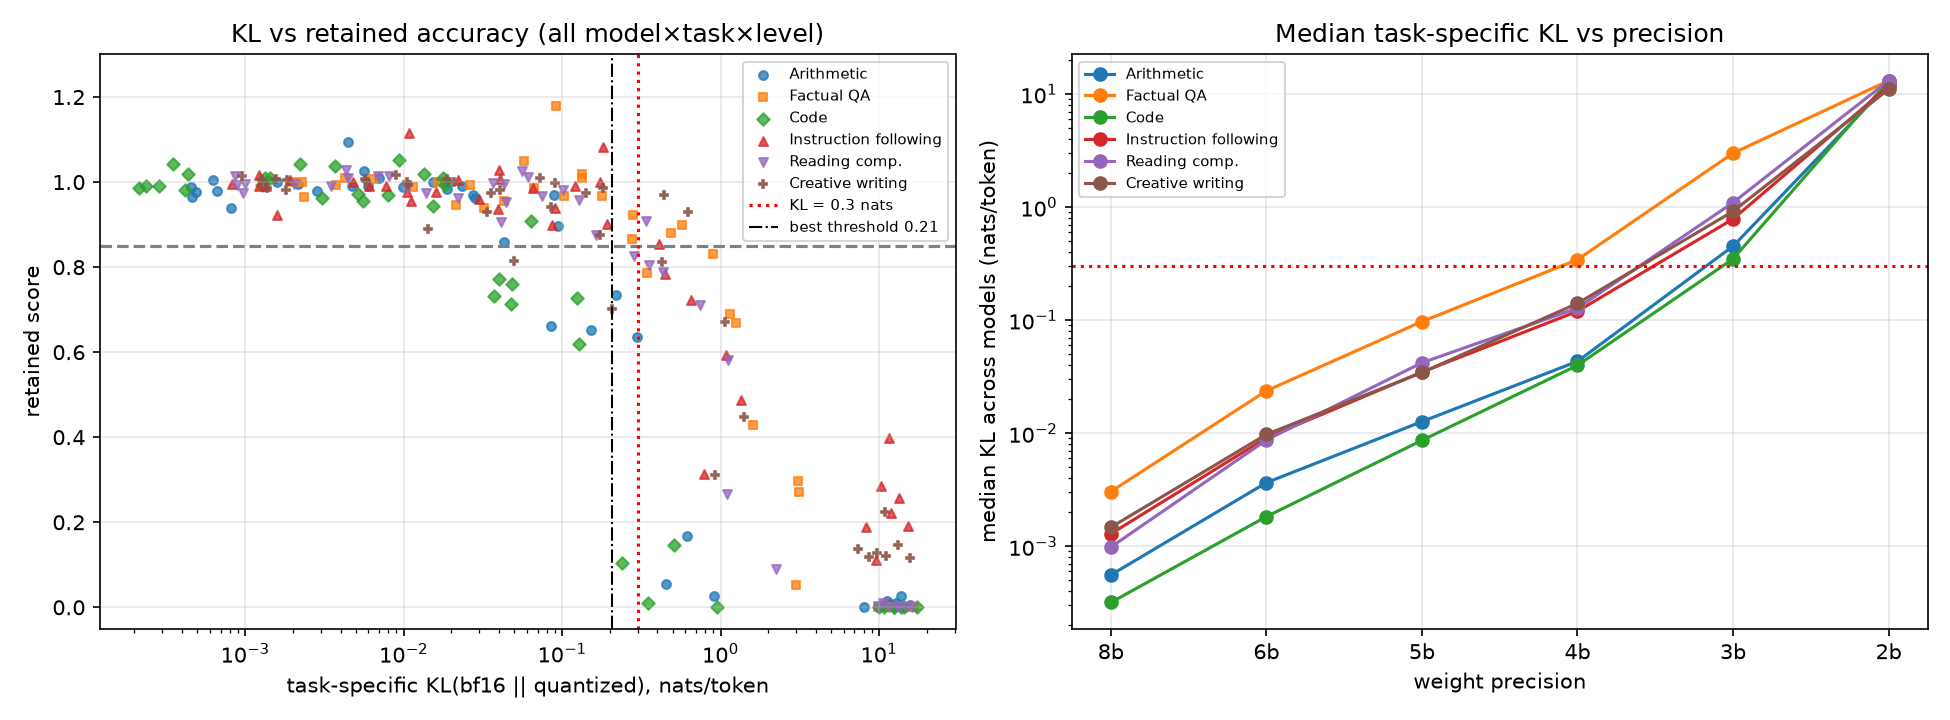
\includegraphics[width=0.95\linewidth]{figures/fig3_kl_vs_accuracy.png}
\caption{\figleft Task-specific KL(bf16\,$\|$\,quantized) vs.\ retained score for every model $\times$ task $\times$ level (log x-axis). The red dotted line marks the hypothesized 0.3 nats, and the dash-dotted line the fitted optimum of 0.21 nats. Broken configurations (below the dashed 0.85 line) mostly lie to the right of the threshold. The exception is a cluster of code failures (green diamonds) at KL $\approx$ 0.04--0.1. \figright Median KL across models grows by roughly $5$--$10\times$ per precision step. Factual QA has the highest KL at every level, and code the lowest.}
\label{fig:kl}
\end{figure}

\begin{table}[t]
\centering
\caption{Median task-specific KL(bf16\,$\|$\,quantized) in nats per token across models. Values at or above the hypothesized 0.3-nat threshold are in \textbf{bold}. Factual QA crosses 0.3 nats at 4 bits even though most models remain healthy there, while code fails at 4 bits for four models with KL below 0.05.}
\label{tab:kl}
\begin{tabular}{@{}lcccccc@{}}
\toprule
\textbf{Task} & \textbf{8 bits} & \textbf{6 bits} & \textbf{5 bits} & \textbf{4 bits} & \textbf{3 bits} & \textbf{2 bits} \\
\midrule
Arithmetic & 0.001 & 0.004 & 0.013 & 0.043 & \textbf{0.45} & \textbf{12.2} \\
Factual QA & 0.003 & 0.024 & 0.097 & \textbf{0.34} & \textbf{3.00} & \textbf{13.1} \\
Code & 0.000 & 0.002 & 0.009 & 0.040 & \textbf{0.35} & \textbf{13.1} \\
Instruction following & 0.001 & 0.009 & 0.035 & 0.120 & \textbf{0.79} & \textbf{11.7} \\
Reading comp. & 0.001 & 0.009 & 0.042 & 0.128 & \textbf{1.10} & \textbf{13.1} \\
Creative writing & 0.001 & 0.010 & 0.034 & 0.141 & \textbf{0.92} & \textbf{11.0} \\
\bottomrule
\end{tabular}
\end{table}

\para{KL is an excellent concurrent detector.} Across 228 quantized model--task--level cells, 85 of them broken, KL correlates strongly with retained score (Spearman $-0.81$). Used as a classifier of broken configurations, KL reaches an AUC of 0.97, compared with 0.98 for the \wikitext perplexity ratio and 0.94 for top-1 agreement. Per-task AUCs range from 0.96 to 1.00. The Youden-optimal threshold is \textbf{0.21 nats (bootstrap 95\% CI 0.12--0.34)}, consistent with the hypothesized $\approx$0.3. At 0.3 nats, sensitivity is 0.84 and specificity 0.96. The result also holds out of sample: on the 60 per-channel cells, which were never used for fitting, KL reaches AUC 0.97, and the 0.3-nat rule has sensitivity 0.82 and specificity 0.92.

\para{KL does not warn early.} For each of the 42 model--task pairs that eventually fall below 0.85, we take the last healthy precision directly above the failing one. There, KL is at least 0.3 nats in only \textbf{6 of 42 cases (14\%)}, with a median of 0.09 nats, and most of these 6 cases are factual QA, where healthy KL is already high. At the failing level itself, KL is at least 0.3 nats in 30 of 42 cases (71\%), with a median of 0.70. KL rises by about $5$--$10\times$ per precision step (\figref{fig:kl}, right), but it crosses 0.3 \emph{together with} the accuracy drop, not before it.

\para{The right threshold varies about $100\times$ across tasks.} \humaneval breaks at very low KL: for the four models whose code cliffs at 4 bits, median KL at the failing level is only 0.04--0.05 nats, because one wrong token can fail the unit tests. \trivia tolerates KL of about 0.3--0.5 nats at healthy levels, because its answers are short and a few high-entropy answer tokens dominate the average (\tabref{tab:kl}). A single 0.3-nat rule therefore misses code failures and over-flags factual QA. The pooled threshold works mostly because KL at 3 and 2 bits is enormous. \textbf{H4 is partially supported}: KL is a strong concurrent signal with a pooled threshold of 0.2--0.3 nats, but it is not a leading indicator, and a pooled threshold is unsafe for code.

\subsection{Ablation: quantization granularity}
\label{sec:granularity}

\begin{table}[t]
\centering
\caption{Mean retained fraction over all six tasks for \qwen-1.5B and \llama-1B, with group-128 vs.\ per-output-channel \rtn. Without group-wise scales the cliff moves up by a full bit: per-channel INT4 (0.62) sits between group-128 INT4 (0.92) and INT3 (0.31). Better (higher) value per row in \textbf{bold}.}
\label{tab:granularity}
\begin{tabular}{@{}lccccc@{}}
\toprule
\textbf{Granularity} & \textbf{8 bits} & \textbf{6 bits} & \textbf{5 bits} & \textbf{4 bits} & \textbf{3 bits} \\
\midrule
Group 128 & 1.00 & \textbf{1.00} & 0.98 & \textbf{0.92} & \textbf{0.31} \\
Per-channel & 1.00 & 0.99 & 0.98 & 0.62 & 0.08 \\
\bottomrule
\end{tabular}
\end{table}

\Tabref{tab:granularity} shows that removing the group-wise scales moves the cliff up by a full bit. At 4 bits, per-channel \rtn retains only 0.62 of bf16 performance on average, compared with 0.92 for group-128. Per-channel INT4 loses 33--57\% on arithmetic, code and factual QA for both models, and \qwen-1.5B's creative-writing score falls to 0.21. ``INT4'' therefore does not name a fixed accuracy level. The scale granularity and the quantizer (\secref{sec:cliff}, \awq) matter as much as the bit count.
